\documentclass[12pt,letterpaper]{article}
\usepackage{listings}
\usepackage{graphicx}
\usepackage[table,xcdraw]{xcolor}
\RequirePackage{xcolor}
\definecolor{tecAzul}{cmyk}{1,0.91,0.33,0.25} % según manual de imagen 2016
\definecolor{tecRojo}{cmyk}{0,0.9,0.86,0}     % según manual de imagen 2016

\renewcommand{\familydefault}{\sfdefault}
\usepackage{amsmath} % for the equation* environment
\usepackage{mwe}
\usepackage{graphicx}
\usepackage[spanish]{babel}
\usepackage{multirow}
\usepackage{titlesec}
\titleformat*{\section}%
{\normalfont\Large\bfseries\color{tecAzul}}
\titleformat*{\subsection}%
{\normalfont\large\bfseries\color{tecAzul}}


\usepackage[tmargin=2cm,bmargin=2cm,lmargin=2.5cm,rmargin=2.5cm]{geometry}
\usepackage{textpos}
\usepackage{tikz}
\usepackage{pgfplots}
\usepackage{pgf}

\usepackage[margin=1cm]{caption}

\usepackage{hyperref}

%
% paragraph layout
%
\parindent0em                           % indentation width of first line
\parskip1.3ex                           % space between paragraphs


\newcommand{\EstudianteA}{David F. Duarte Sánchez}

\pgfplotsset{compat=1.17}



\usepackage{listings}
\usepackage{xcolor}

\definecolor{codegreen}{rgb}{0,0.6,0}
\definecolor{codegray}{rgb}{0.5,0.5,0.5}
\definecolor{codepurple}{rgb}{0.58,0,0.82}
\definecolor{backcolour}{rgb}{0.95,0.95,0.92}

\lstdefinestyle{mystyle}{
    backgroundcolor=\color{backcolour},   
    commentstyle=\color{codegreen},
    keywordstyle=\color{magenta},
    numberstyle=\tiny\color{codegray},
    stringstyle=\color{codepurple},
    basicstyle=\ttfamily\footnotesize,
    breakatwhitespace=false,         
    breaklines=true,                 
    captionpos=b,                    
    keepspaces=true,                 
    numbers=left,                    
    numbersep=5pt,                  
    showspaces=false,                
    showstringspaces=false,
    showtabs=false,                  
    tabsize=2
}

\lstset{style=mystyle}



\begin{document}
	
\graphicspath{{./}{./fig/}}

%-------------------------- Title section -------------------------------------%

%
\begin{textblock}{10}[0,0](-0.5,0)
	\large Escuela de Ingeniería Electrónica \\ 
	EL5617 Trabajo Final de Graduación \\
\end{textblock}

%
\begin{textblock}{10}[0,0](2.6,-0.35)
	\begin{flushright}
		
\includegraphics[scale=0.8]{Firma_TEC-4.pdf}
	\end{flushright}
\end{textblock}

%% Title %%
\begin{center}
	\vspace{70mm}
	{\large\color{tecRojo} Trabajo Final de Graduación}
	\par\vspace{8mm}
	{\Large\bf\color{tecAzul}{Bitácora de Trabajo - Entrega 2}}
	\par\vspace{100mm}
	{{\EstudianteA \\ II Semestre 2024} 
	\vspace{8mm}}
\end{center}

\newpage
%------------------------------------------------------------------------------%

\renewcommand{\baselinestretch}{1.1}    % line spacing

%------------------------------------------------------------------------------%

\section{Semana 7}
\subsection{Corrección de anteproyecto}

\bf{Fecha de trabajo:} 23/08/2024.\\
\bf{Objetivo:} Corrección de observaciones realizadas a la Tesis.

\begin{table}[h!]
    \label{tab:my-tables}
    \resizebox{\textwidth}{!}{%
    \begin{tabular}{|l|}
        \hline
        \hline
        \multicolumn{1}{|c|}{Reporte de   actividades} \\ \hline
        \hline
        - Restructuración de la sección de marco teórico, se acuerda que el mismo será \\
        compuesto por no más de 10 páginas, en las cuales se hablara de temas como lo son \\
        ¿Qué es la estimación?, ¿Qué es el control?, ¿Que son los procesadores embebidos?\\
        ¿Qué es un marco de trabajo?, ¿Qué es el model to model transformation? y ¿Que es \\
        el código embebido?, además de esto se estructura una revisión literaria no mayor a \\
        4 años de antigüedad y el estado del arte. \\ \hline
        
        - Se trata de evitar mencionar mucho el tema de control automático en la tesis, esto con \\
        el fin de evitar que el lector crea que es una tesis que se basara en realizar control \\
        automático, si no que más bien quede claro desde el inicio que se trabajara en \\
        sistemas embebidos que deberán de correr los modelos de control que ya nos den desarrollados \\ \hline
        
        - Finalmente se revisa la presentación que se presentara a los profesores asesores, a los cuales \\
        se les presentara la propuesta de anteproyecto con el fin de obtener realimentación por parte de \\
        ellos y asi mejorar la propuesta antes de la evaluación de la misma. \\ \hline

        - Se establece como marco de trabajo a utilizar Yocto Project y se comienza a buscar la forma de \\
        encontrar una distribución de linux la cual pueda soportar el modelo de board support package \\
        con el cual se deberá de generar la solución. \\ \hline\hline
        
        \hline
        \multicolumn{1}{|c|}{Productos obtenidos} \\ \hline\hline
        Se comienza a trabajar en la reestructuración del marco teórico usando las preguntas \\
        mencionadas anteriormente como generadores, esto con el fin de aclarar al lector \\
        algunos de los conceptos básicos que va a requerir para poder comprender el hilo \\
        conductor del trabajo escrito.\\

        El tema de control eléctrico se menciona de forma muy superficial en la tesis,\\
        solamente se explica que es el control automático y porque es de relevancia en\\
        el desarrollo de esta tesis, pero se explica de forma explícita que el conjunto \\
        de flujos de trabajo a desarrollar en esta tesis se encontraran ubicados en el \\
        medio más no serán parte física del control eléctrico realizado.\\
        
        Además por otro lado se comienza a trabajar en el primer capítulo de la tesis en\\
        donde se debe de seleccionar el número de parte de la tarjeta de desarrollo con\\
        la cual se plantea el desarrollo del proyecto, se establece el uso de la tarjeta de \\
        desarrollo Zeadbord, la cual deberá de trabajar bajo el marco de trabajo de Yocto, \\
        para esto se deberá de seguir el manual que se adjunta. \\ \hline \hline  
    \end{tabular}}
\end{table}

Como se mencionó anteriormente se logró encontrar un BSP disponible para la ZeadBoard, el mismo
se encuentra actualmente disponible para la distribución de Yocto Zeus la cual tuvo el lanzamiento 
en el año de 2019, por tanto es necesario instalar Ubuntu 18.04 para poder llevar a cabo la elaboración
del conjunto de flujos de trabajo. Los mismos se realizan siguiendo esta serie de pasos. 

Tabla con las versiones de Yocto

\begin{table}[h!]
    \caption{}
    \label{tab:my-table}
    \resizebox{\textwidth}{!}{%
    \begin{tabular}{|l|l|l|l|l|l|l|}
    \hline
    \rowcolor[HTML]{EAECF0} 
    \multicolumn{1}{|c|}{\cellcolor[HTML]{EAECF0}{\color[HTML]{202122} \textbf{Codename}}} &
      \multicolumn{1}{c|}{\cellcolor[HTML]{EAECF0}{\color[HTML]{202122} \textbf{Yocto Project Version}}} &
      \multicolumn{1}{c|}{\cellcolor[HTML]{EAECF0}{\color[HTML]{202122} \textbf{Release Date}}} &
      \multicolumn{1}{c|}{\cellcolor[HTML]{EAECF0}{\color[HTML]{202122} \textbf{Current Version}}} &
      \multicolumn{1}{c|}{\cellcolor[HTML]{EAECF0}{\color[HTML]{202122} \textbf{Support Level}}} &
      \multicolumn{1}{c|}{\cellcolor[HTML]{EAECF0}{\color[HTML]{202122} \textbf{Poky Version}}} &
      \multicolumn{1}{c|}{\cellcolor[HTML]{EAECF0}{\color[HTML]{202122} \textbf{BitBake branch}}} \\ \hline
    \rowcolor[HTML]{F8F9FA} 
    {\color[HTML]{708090} Zeus} &
      {\color[HTML]{708090} 3.0} &
      {\color[HTML]{708090} October 2019} &
      {\color[HTML]{708090} 3.0.4 (August 2020)} &
      {\color[HTML]{708090} EOL} &
      {\color[HTML]{708090} 22.0.3} &
      {\color[HTML]{708090} 1.44} \\ \hline
    \rowcolor[HTML]{F8F9FA} 
    {\color[HTML]{708090} Dunfell} &
      {\color[HTML]{708090} 3.1} &
      {\color[HTML]{708090} April 2020} &
      {\color[HTML]{708090} 3.1.33 (May 2024)} &
      {\color[HTML]{708090} EOL - LTS¹} &
      {\color[HTML]{708090} 23.0} &
      {\color[HTML]{708090} 1.46} \\ \hline
    \end{tabular}%
    }
    \end{table}
Tabla con las versiones de bsp según el repo de xilinx

\begin{figure}[h!]
  \centering
  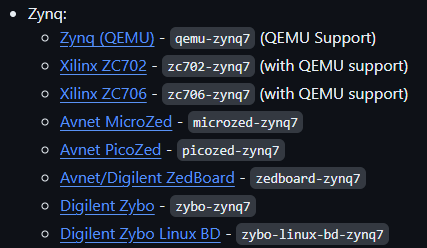
\includegraphics{images/image01.png}
  \caption{BSP Xilinx}
  \label{fig:Entorno}
\end{figure}


Indicar que se sigue bajo la investigación si hay alguna versión lts que soporte el zedboard

\begin{lstlisting}[language=bash]
sudo apt-get install gawk wget git-core diffstat unzip texinfo 
gcc-multilib build-essential chrpath socat cpio python python3 
python3-pip python3-pexpect xz-utils debianutils iputils-ping 
python3-git python3-jinja2 libegl1-mesa libsdl1.2-dev pylint3
xterm

git clone -b zeus https://git.yoctoproject.org/git/poky
cd poky

git clone -b zeus https://github.com/Xilinx/meta-xilinx
git clone -b zeus https://github.com/openembedded/meta-openembedded.git

source oe-init-build-env

echo "MACHINE??=\"zedboard-zynq7\"" >> conf/local.conf
echo "IMAGE_FEATURES += \"package-management\"" >> conf/local.conf
echo "DISTRO_HOSTNAME = \"zynq\"" >> conf/local.conf

bitbake-layers add-layer ../meta-xilinx/meta-xilinx-bsp/
bitbake-layers add-layer ../meta-openembedded/meta-oe/

bitbake core-image-minimal
\end{lstlisting}

De momento se trabaja la versión encontrada con Yocto Zeus, con el fin de generar una imagen mínima y comenzar
con el trabajo de adaptación.

%\bibliography{bibliografia_consultada}
%\bibliographystyle{plain}
\end{document}